\documentclass[tikz,border=2pt]{standalone}
\usetikzlibrary{arrows.meta,positioning,calc,shapes.geometric}
\usepackage{fontspec}
\setmainfont{TeX Gyre Termes}
\setsansfont{Roboto}
\begin{document}
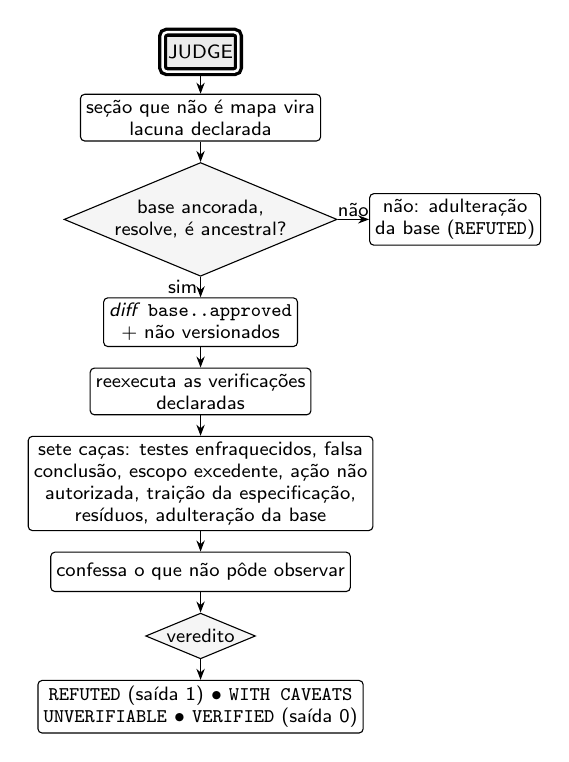
\begin{tikzpicture}[
  font=\sffamily\scriptsize, >={Stealth[length=4pt]},
  proc/.style={draw, thin, rounded corners=1.5pt, align=center, fill=white, minimum height=0.5cm, inner sep=2pt},
  exec/.style={proc, very thick, double distance=0.9pt, fill=black!8},
  dec/.style={draw, thin, diamond, aspect=2.4, align=center, fill=black!4, inner sep=0.5pt, font=\sffamily\scriptsize},
  nota/.style={font=\sffamily\scriptsize, align=center, text=black!80},
  lbl/.style={font=\sffamily\scriptsize, inner sep=1pt}
]
\node[exec] (a) {JUDGE};
\node[proc, below=0.26cm of a] (norm) {seção que não é mapa vira\\ lacuna declarada};
\node[dec, below=0.26cm of norm] (base) {base ancorada,\\ resolve, é ancestral?};
\node[proc, right=0.4cm of base] (tamp) {não: adulteração\\ da base (\texttt{REFUTED})};
\node[proc, below=0.26cm of base] (diff) {\textit{diff} \texttt{base..approved}\\ + não versionados};
\node[proc, below=0.26cm of diff] (re) {reexecuta as verificações\\ declaradas};
\node[proc, below=0.26cm of re] (hunt)
  {sete caças: testes enfraquecidos, falsa\\
   conclusão, escopo excedente, ação não\\
   autorizada, traição da especificação,\\
   resíduos, adulteração da base};
\node[proc, below=0.26cm of hunt] (blind) {confessa o que não pôde observar};
\node[dec, below=0.26cm of blind] (v) {veredito};
\node[proc, below=0.26cm of v] (out)
  {\texttt{REFUTED} (saída 1) $\bullet$ \texttt{WITH CAVEATS}\\
   \texttt{UNVERIFIABLE} $\bullet$ \texttt{VERIFIED} (saída 0)};
\draw[->] (a) -- (norm);
\draw[->] (norm) -- (base);
\draw[->] (base) -- node[lbl,above]{não} (tamp);
\draw[->] (base) -- node[lbl,left]{sim} (diff);
\draw[->] (diff) -- (re);
\draw[->] (re) -- (hunt);
\draw[->] (hunt) -- (blind);
\draw[->] (blind) -- (v);
\draw[->] (v) -- (out);
\end{tikzpicture}
\end{document}
